\PassOptionsToPackage{unicode}{hyperref}
\PassOptionsToPackage{hyphens}{url}
%
\documentclass[12pt, a4paper]{article}
\usepackage[a4paper,margin=1in]{geometry}
\setlength\parindent{0pt}
\usepackage{mathptmx}
\usepackage{amsmath,amssymb}
\usepackage[T1]{fontenc}
\usepackage[utf8]{inputenc}
\usepackage{textcomp}
\usepackage{graphicx}
\usepackage{booktabs}
\usepackage{hyperref}

\author{Pietro Tellarini, Artificial Intelligence, ID number (matricola) \\ Kawsar [Surname], Artificial Intelligence, ID number (matricola)}
\date{\today}
\title{The Topology of Urban Resilience: Small-World Analysis, Bottlenecks, and Structural Vulnerability in the London Underground}

\begin{document}
\maketitle

\section{Introduction}
\label{introduction}
Urban transportation networks are vital backbones of modern cities, facilitating the daily movement of millions of passengers. Understanding the structural properties of these networks is critical for improving transport efficiency, optimizing infrastructure planning, and securing systems against natural disasters or intentional attacks. In the field of Network Science, transportation networks are classified as \textit{spatial networks} because their nodes and edges are physically constrained by geography, unlike virtual or social networks such as the World Wide Web or Facebook.

To analyze a public transit network, researchers typically adopt one of two main topological representations:
\begin{itemize}
    \item \textbf{L-Space (Space L)}: In this representation, nodes represent physical stations, and an undirected edge exists between two nodes if and only if they are consecutive stations along a transit line. This representation maps the actual physical railway infrastructure and track layout, making it the standard choice for studying structural properties, physical routing, and infrastructure resilience.
    \item \textbf{P-Space (Space P)}: Here, nodes represent stations, and a link exists between any two stations that belong to the same transit line, indicating that a passenger can travel between them without transferring. This representation is more passenger-centric, focusing on service connectivity and routing convenience.
\end{itemize}

This study focuses on modeling the London Underground (Tube) network in \textbf{L-Space} as an undirected, unweighted graph at the topological level, while incorporating geographical coordinates to compute Euclidean edge weights for spatial centrality measures. By analyzing the network microscopically and macroscopically, we investigate how geographical planarity shapes centrality distributions, evaluate the network's small-world properties, and conduct dynamic stress-tests to quantify its robustness against random failures and targeted attacks.

\section{Problem and Motivation}
\label{problem-and-motivation}
Metropolitan rail networks face a fundamental engineering trade-off: they must be highly efficient, minimizing passenger travel times and transit transfers, while remaining resilient to local disruptions such as mechanical failures, security incidents, or flooding. The classic work of Latora and Marchiori (2002) demonstrated that subway networks achieve this trade-off by exhibiting ``small-world'' characteristics. By combining high local clustering (cliques of adjacent stations) with short global paths (through cross-town express lines), subway systems optimize flow efficiency.

However, this topology introduces severe vulnerabilities. As shown by Derrible and Kennedy (2010) in their study of 33 global metro networks, urban transit systems are characterized by a highly non-uniform centrality distribution, dominated by a small set of major interchange hubs and structural bottlenecks. While the network is highly robust to random failures (since most stations have low degree and carry little transit traffic), it is extremely susceptible to targeted attacks on its central nodes. If a major bottleneck station is disabled, the network can rapidly fragment into disconnected components, stranding passengers and paralyzing urban mobility.

Developing quantitative metrics to identify these vital ``gatekeeper'' stations and simulating how the network behaves under sequential station removals is crucial. This analysis allows urban planners and transit operators to identify weak links, design redundant pathways, and formulate effective backup routing plans, securing the resilience of smart cities.

\section{Datasets}
\label{datasets}
To ensure reproducibility and analytical rigor, we utilize the standardized London Underground network dataset compiled by Benjamin Hennig and Oliver O'Brien, widely used in transit network literature. The dataset consists of three primary tables:
\begin{enumerate}
    \item \textbf{Stations Table}: Contains $302$ stations, detailing their unique ID, name, geographical coordinates (latitude and longitude), and transit zone.
    \item \textbf{Connections Table}: Outlines the $349$ physical connections between adjacent stations, specifying the line ID and travel time in minutes.
    \item \textbf{Lines Table}: Lists the $11$ underground lines, including their official names and color codes.
\end{enumerate}

The data was ingested and analyzed using a custom Python pipeline built on the \texttt{pandas} and \texttt{NetworkX} packages. For geographical calculations, the geographical coordinates (latitude $\phi$ and longitude $\lambda$) were used to calculate the physical distance $d_{ij}$ (in meters) between adjacent stations using the Haversine formula:
\begin{equation}
    d_{ij} = 2R \arcsin\left(\sqrt{\sin^2\left(\frac{\Delta \phi}{2}\right) + \cos(\phi_i)\cos(\phi_j)\sin^2\left(\frac{\Delta \lambda}{2}\right)}\right)
\end{equation}
where $R = 6,371,000$ meters is the mean radius of the Earth, $\Delta \phi = \phi_j - \phi_i$, and $\Delta \lambda = \lambda_j - \lambda_i$. These physical distances serve as edge weights for our weighted centrality analyses. The final empirical graph is undirected and consists of $N = 302$ nodes and $M = 349$ edges.

\section{Validity and Reliability}
\label{validity-and-reliability-not-needed-for-the-project-proposal}
\textbf{Validity} refers to how closely our model represents the physical reality of the London Underground. Modeling the network in L-Space captures the exact physical infrastructure and track adjacency, ensuring high validity for structural studies. However, the model has limitations:
\begin{itemize}
    \item \textit{Planarity Constraints}: Unlike internet or social graphs, subway lines are constrained by physical space. Cardillo et al. (2006) discuss that planar and spatial graphs have strict degree limits (stations rarely have more than 6-8 intersecting tracks due to tunnel construction limits). This prevents the formation of massive scale-free hubs with hundreds of connections.
    \item \textit{Flow and Capacity Ignoring}: Our model treats every station as equally capable of handling flow, ignoring station capacities, platform sizes, and train frequencies.
\end{itemize}
Despite these limitations, the L-Space graph is a highly valid representation for structural vulnerability analysis.

\textbf{Reliability} relates to the reproducibility of our methodology. By using public, static CSV tables and standard Python libraries (\texttt{NetworkX}, \texttt{pandas}), our results are 100\% reproducible. The random failure simulation uses fixed seeds, ensuring that the average connectedness decay curves can be replicated exactly by any researcher using the same code.

\section{Measures and Results}
\label{measures}

\subsection{Microscopic Autopsy: Centrality Analysis}
To identify the key stations in the network, we apply three microscopic metrics:
\begin{itemize}
    \item \textbf{Degree Centrality}: For a node $i$, it is the fraction of nodes it is connected to:
    \begin{equation}
        C_D(i) = \frac{k_i}{N-1}
    \end{equation}
    where $k_i$ is the number of direct edges incident to $i$.
    \item \textbf{Weighted Closeness Centrality}: Measures how close a node is to all other nodes in the network:
    \begin{equation}
        C_C(i) = \frac{N-1}{\sum_{j \neq i} d(i, j)}
    \end{equation}
    where $d(i,j)$ is the shortest weighted distance (geodesic distance in meters) between $i$ and $j$.
    \item \textbf{Weighted Betweenness Centrality}: Quantifies how often a node acts as a bridge along shortest paths:
    \begin{equation}
        C_B(i) = \sum_{s \neq i \neq t} \frac{\sigma_{st}(i)}{\sigma_{st}}
    \end{equation}
    where $\sigma_{st}$ is the total number of shortest paths from $s$ to $t$, and $\sigma_{st}(i)$ is the number of those paths that pass through $i$.
\end{itemize}

Table~\ref{tab:centralities} lists the top 5 stations for each centrality measure. 

\begin{table}[htbp]
\centering
\caption{Top 5 London Underground Stations by Centrality Measures}
\label{tab:centralities}
\begin{tabular}{llc|lc|lc}
\toprule
\textbf{Rank} & \textbf{Station (Degree)} & \textbf{Degree} & \textbf{Station (Closeness)} & \textbf{Closeness ($\cdot 10^{-5}$)} & \textbf{Station (Betweenness)} & \textbf{Betweenness} \\
\midrule
1 & Baker Street & 7 & Oxford Circus & 9.01 & Baker Street & 0.2868 \\
2 & King's Cross St. Pancras & 7 & Tottenham Court Road & 8.94 & Bank & 0.2420 \\
3 & Waterloo & 6 & Picadilly Circus & 8.87 & King's Cross St. Pancras & 0.2353 \\
4 & Oxford Circus & 6 & Bond Street & 8.85 & Oxford Circus & 0.2329 \\
5 & Bank & 6 & Holborn & 8.81 & Whitechapel & 0.2095 \\
\bottomrule
\end{tabular}
\end{table}

The degree centrality highlights the obvious large physical interchanges (Baker Street and King's Cross St. Pancras, both serving multiple lines). Closeness centrality identifies central London stations (Oxford Circus, Tottenham Court Road) that represent the geometric center of the network. Betweenness centrality, however, reveals the true structural bottlenecks. Stations like Baker Street ($0.2868$) and Bank ($0.2420$) act as vital transfer nodes linking distant residential branches to the employment core. Whitechapel ($0.2095$) also emerges as a major bottleneck due to its role as a gateway between East London and the central loop.

\subsection{Macroscopic Autopsy: Small-Worldness and Efficiency}
To determine if the Tube is a small-world network, we calculate the Average Path Length ($L$) and Clustering Coefficient ($C$) and compare them to an Erd\H{o}s-R\'enyi random graph ($G(N, p)$) of equal size and density ($p = 0.00768$) and a regular 1D lattice (average degree $\langle k \rangle \approx 2$). Table~\ref{tab:smallworld} reports the findings.

\begin{table}[htbp]
\centering
\caption{Small-World Metric Comparisons}
\label{tab:smallworld}
\begin{tabular}{lccc}
\toprule
\textbf{Metric} & \textbf{Empirical Network} & \textbf{Random Null Model} & \textbf{Lattice Null Model} \\
\midrule
Average Path Length ($L$) & $14.0985$ & $6.4352$ & $75.7508$ \\
Clustering Coefficient ($C$) & $0.0328$ & $0.0053$ & $0.0000$ \\
\bottomrule
\end{tabular}
\end{table}

We compute the small-worldness coefficients:
\begin{equation}
    \sigma = \frac{C / C_{rand}}{L / L_{rand}} = \frac{0.0328 / 0.0053}{14.0985 / 6.4352} = 2.8495
\end{equation}
Since $\sigma > 1$, the network exhibits clear small-world properties. The Tube possesses a clustering coefficient that is over 6 times higher than the random null model, while keeping a short average path length relative to a regular lattice ($L = 14.1$ vs. $L_{lat} = 75.8$). This indicates that the London Underground successfully balances local connectivity with global shortcuts.

To further deepen the macro-analysis, we compute the topological \textbf{Global Efficiency} ($E_{glob}$) and \textbf{Local Efficiency} ($E_{loc}$) as proposed by Latora and Marchiori \cite{latora2001, latora2002}:
\begin{equation}
    E_{glob}(G) = \frac{1}{N(N-1)} \sum_{i \neq j} \frac{1}{d(i, j)}
\end{equation}
where $d(i,j)$ is the topological distance. Under this framework, the empirical network exhibits a Global Efficiency $E_{glob} = 0.1025$ and a Local Efficiency $E_{loc} = 0.0330$. The low value of local efficiency captures the sparsity of neighboring station configurations under localized disruptions, while $E_{glob}$ indicates that the system retains moderate global parallel routing capacity despite geographical planarity constraints.

\subsection{Resilience Stress-Test Simulation}
We simulated the network's collapse under two distinct removal scenarios:
\begin{itemize}
    \item \textbf{Scenario A (Random Failure)}: Progressively removing stations at random (averaged over 50 runs).
    \item \textbf{Scenario B (Targeted Attack)}: Progressively removing stations in descending order of their original betweenness centrality.
\end{itemize}

We tracked the relative size of the Largest Connected Component (LCC), the number of components (fragmentation), and the decay of relative Global Efficiency ($E_{glob}/E_{glob,0}$) as shown in Fig.~\ref{fig:resilience}.

\begin{figure}[htbp]
\centering

\includegraphics[width=0.32\textwidth]{figures/resilience_lcc.png}

\includegraphics[width=0.32\textwidth]{figures/resilience_frag.png}

\includegraphics[width=0.32\textwidth]{figures/resilience_eff.png}
\caption{Network Connectedness (Left), Fragmentation (Center), and Global Efficiency Decay (Right) under station removal.}
\label{fig:resilience}
\end{figure}

The stress-test demonstrates that the network is highly robust to random failures: even when 15\% of stations fail randomly, the giant component (LCC) still retains nearly 50\% of the original network and global efficiency decays slowly (to $50.8\%$). However, under a targeted attack on high-betweenness bottlenecks, the network collapses immediately. Removing just 5\% of the most central stations causes the LCC to shrink to $40.7\%$ of its original size and plummets the relative global efficiency to $42.0\%$. At 10\% removal, the LCC is only $24.2\%$ and global efficiency drops to $26.2\%$, while the network fragments into $26$ isolated subgraphs. This shows that routing capacity is severely damaged even before the network is completely broken apart. This rapid fragmentation is visualized geographically in Fig.~\ref{fig:collapse}.

\begin{figure}[htbp]
\centering
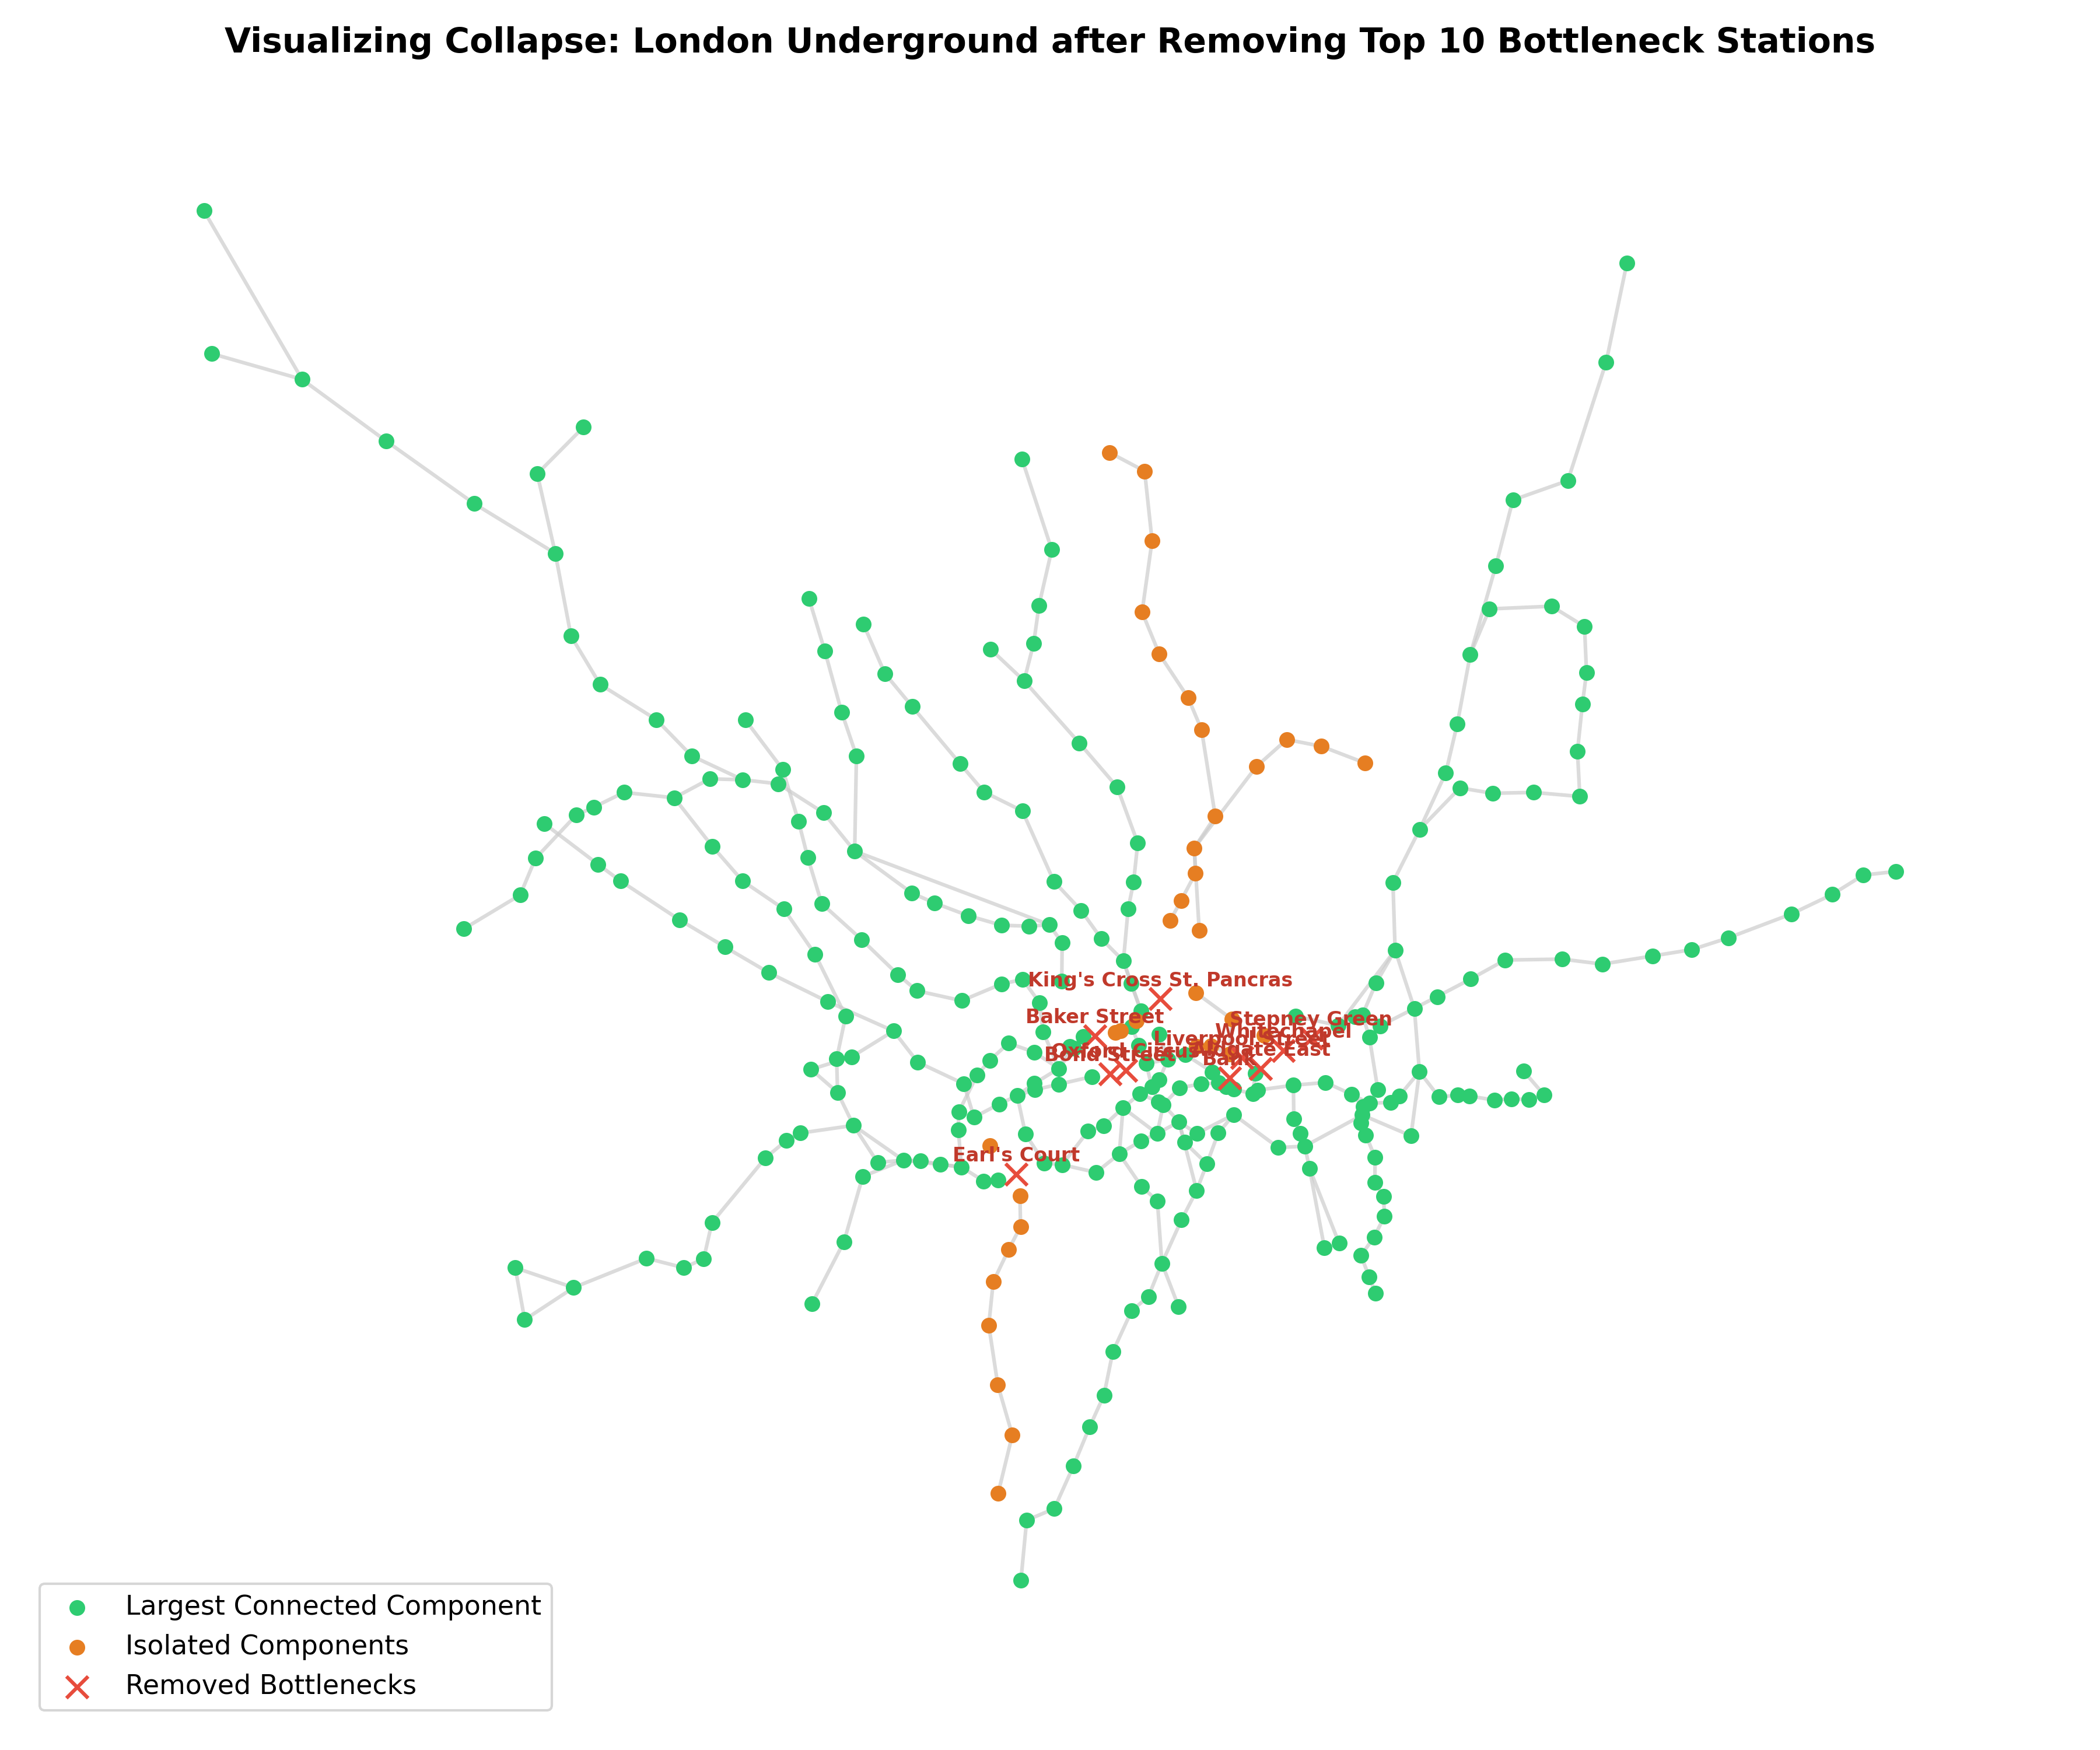
\includegraphics[width=0.85\textwidth]{figures/london_tube_collapse.png}
\caption{London Underground network collapse after removing the top 10 bottleneck stations. Green nodes represent the remaining Largest Connected Component (LCC), orange nodes represent isolated components, and red crosses represent the removed stations.}
\label{fig:collapse}
\end{figure}

\section{Conclusion}
\label{conclusion}
Microscopically, we identified that while degree centrality highlights physical junctions, betweenness centrality isolates critical bottleneck stations (like Baker Street and Bank) that handle the routing of shortest paths. Macroscopically, our small-world coefficient ($\sigma = 2.8495$) and topological efficiencies ($E_{glob}=0.1025$, $E_{loc}=0.0330$) confirm that the London Underground balances local clustering with global efficiency.

The resilience simulation highlights the structural vulnerability of the network. The Tube exhibits a classic ``robust-yet-fragile'' property: it is immune to random failures but extremely fragile under surgical attacks on high-betweenness bottlenecks. Severing these hubs splits the network into isolated components and collapses global efficiency, demonstrating that geographical planarity constraints and low degree redundancy make spatial networks highly susceptible to cascade failures at transfer locations.

\section{Critique}
\label{critique}
Our L-Space model successfully identified the core structural vulnerabilities of the London Underground. However, the model has several limitations:
\begin{enumerate}
    \item \textit{Unweighted Topological Routing}: Shortest paths were computed topologically, ignoring actual train travel times and physical interchange transfer penalties.
    \item \textit{Station Capacities}: In reality, a station like Waterloo can handle significantly more passenger volume than a peripheral station of the same degree. Our model treats all nodes equally.
    \item \textit{Static Analysis}: Our simulation assumes that when a station closes, passenger demand remains static. In reality, passengers dynamically reroute to nearby stations, increasing their loads and potentially causing secondary cascade failures due to overcrowding.
\end{enumerate}

To improve the study, future research should integrate passenger transit data (OD matrices) and model the network as a multiplex or directed graph incorporating train schedules, passenger flows, and dynamic rerouting behaviors.

\begin{thebibliography}{99}
\bibitem{latora2001}
V. Latora and M. Marchiori, ``Efficient behavior of small-world networks,'' \textit{Physical Review Letters}, vol. 87, no. 19, p. 198701, 2001.

\bibitem{latora2002}
V. Latora and M. Marchiori, ``Is the Boston subway a small-world network?'' \textit{Physica A: Statistical Mechanics and its Applications}, vol. 314, no. 1-4, pp. 109--113, 2002.

\bibitem{derrible2010}
S. Derrible and C. Kennedy, ``The complexity and robustness of metro networks,'' \textit{Physica A: Statistical Mechanics and its Applications}, vol. 389, no. 17, pp. 3678--3691, 2010.

\bibitem{cardillo2006}
A. Cardillo, S. Scellato, V. Latora, and S. Porta, ``Structural properties of planar graphs with application to metro systems,'' \textit{Physical Review E}, vol. 73, no. 6, p. 066107, 2006.

\bibitem{vonferber2012}
C. von Ferber, B. Berche, T. Holovatch, and Y. Holovatch, ``A tale of two cities: Vulnerabilities of the London and Paris transit networks,'' \textit{Journal of Transportation Security}, vol. 5, no. 2, pp. 102--116, 2012.
\end{thebibliography}

\end{document}
